\chapter{BACKGROUND}
% CONSISTENCY CHECKS
%   - pretraining NOT pre-training
%   - fine-tuning NOT finetuning



% ***************************************************
% SECTION 1
% ***************************************************
\section{The Automatic Speech Recognition Task}\label{sec:background}
Speech recognition or automatic speech recognition (ASR) is the task of 
predicting the text, sentence, transcription, or sequence of characters 
for a corresponding speech recording.
The general approach of ASR is to first compute feature representations called \emph{speech features} from given audio data,
and then map the speech features to characters or other tokens such as wordpieces.



\subsection{Speech recognition data}
The first step of creating an ASR model is to prepare the data that is used for the model.
A single data entry for an ASR dataset is a speech recording (typically in waveform audio file format)
along with a corresponding text transcription of the words which are spoken.
We explain why the choice of dataset has a significant effect on the accuracy of ASR models.

\paragraph*{The amount of training data.} The more data that is available during training the better the ability
of the ASR model to generalize. A small dataset (with few unique voices) may lead to overfitting to the specific 
voices in the dataset.
\paragraph*{The difference between read and conversational speech.} Humans tend to pronounce their speech more clearly 
when reading text from a transcript, and recent ASR models can predict read speech very accurately \cite{jurafskyspeech}.
In contrast, accurately predicting conversational speech is still a major challenge in ASR.
\paragraph*{Tonal qualities for different accents.} The accent of the speaker, which depends on the gender, 
age and ethnicity of the speaker is another important factor to bare in mind. Generally, male speakers
have a lower pitch compared to female speakers. Similarly, adult voices are generally have a lower pitch
compared to children.
\paragraph*{The audio quality of speech recordings.} The position of the microphone, the quality of the microphone, 
the number of microphones available, and the presence of background noise contribute towards the quality of speech recordings.



\subsection{Speech features}
Computing speech features is useful because audio data consists of a one-dimensional array of integers that describe the
amplitude of the recorded sound wave for small time periods called \emph{samples} (see Figure~\ref{}). 
The issue is that mapping a sequence of amplitude measurements to a sequence of characters is impractical. 
A common technique used to compute speech features is to transform the audio data from the amplitude-time domain 
to the frequency-time domain, using the Fast Fourier Transform (FFT) algorithm \cite{cochran1967fast}, \cite{cooley1969fast}.
However, in this study we discuss a more recent feature extraction approach based on contrastive learning.



% ***************************************************
% SECTION 2
% ***************************************************
\section{wav2vec 2.0}
wav2vec 2.0 provides a framework for learning speech representations using unlabeled speech data.
wav2vec 2.0 can be applied to a variety of speech-related tasks such as speech recognition, speech translation,
and speech classification.
It has proved to be particularly useful in cases where a lot of unlabeled data is available, but not much labeled data is available.
The authors show that using just ten minutes of labeled data and pretraining
on $53$k hours of unlabeled data still achieves $4.8$/$8.2$ WER on the clean/other test sets of Librispeech~\cite{}.

The general two-step approach for using wav2vec 2.0 for any speech-related task is the following.
First train (or ``pre-train'') the wav2vec 2.0 model on a large corpus of unlabeled data, which
will give you a model that converts audio data into speech features.
After pretraining, fine-tune the wav2vec 2.0 model for speech recognition using a much smaller corpus of labeled data. 
Fine-tuning wav2vec 2.0 for speech recognition involves replacing the head of the pretrained model with
an appropriate loss function such as CTC.

The wav2vec 2.0 architecture is described by the network diagram in Figure~\ref{wav2vec2_architecture}.
There are three important components of the wav2vec 2.0 architecture:
the feature-encoder, the quantization module, and the context network.
The objective of wav2vec 2.0 becomes clear only after understanding each of the three
components. Thus, the way in which wav2vec 2.0 is trained is only explained after discussing
the three components in detail.

\begin{figure}
    \centering
    \captionsetup{justification=centering}
    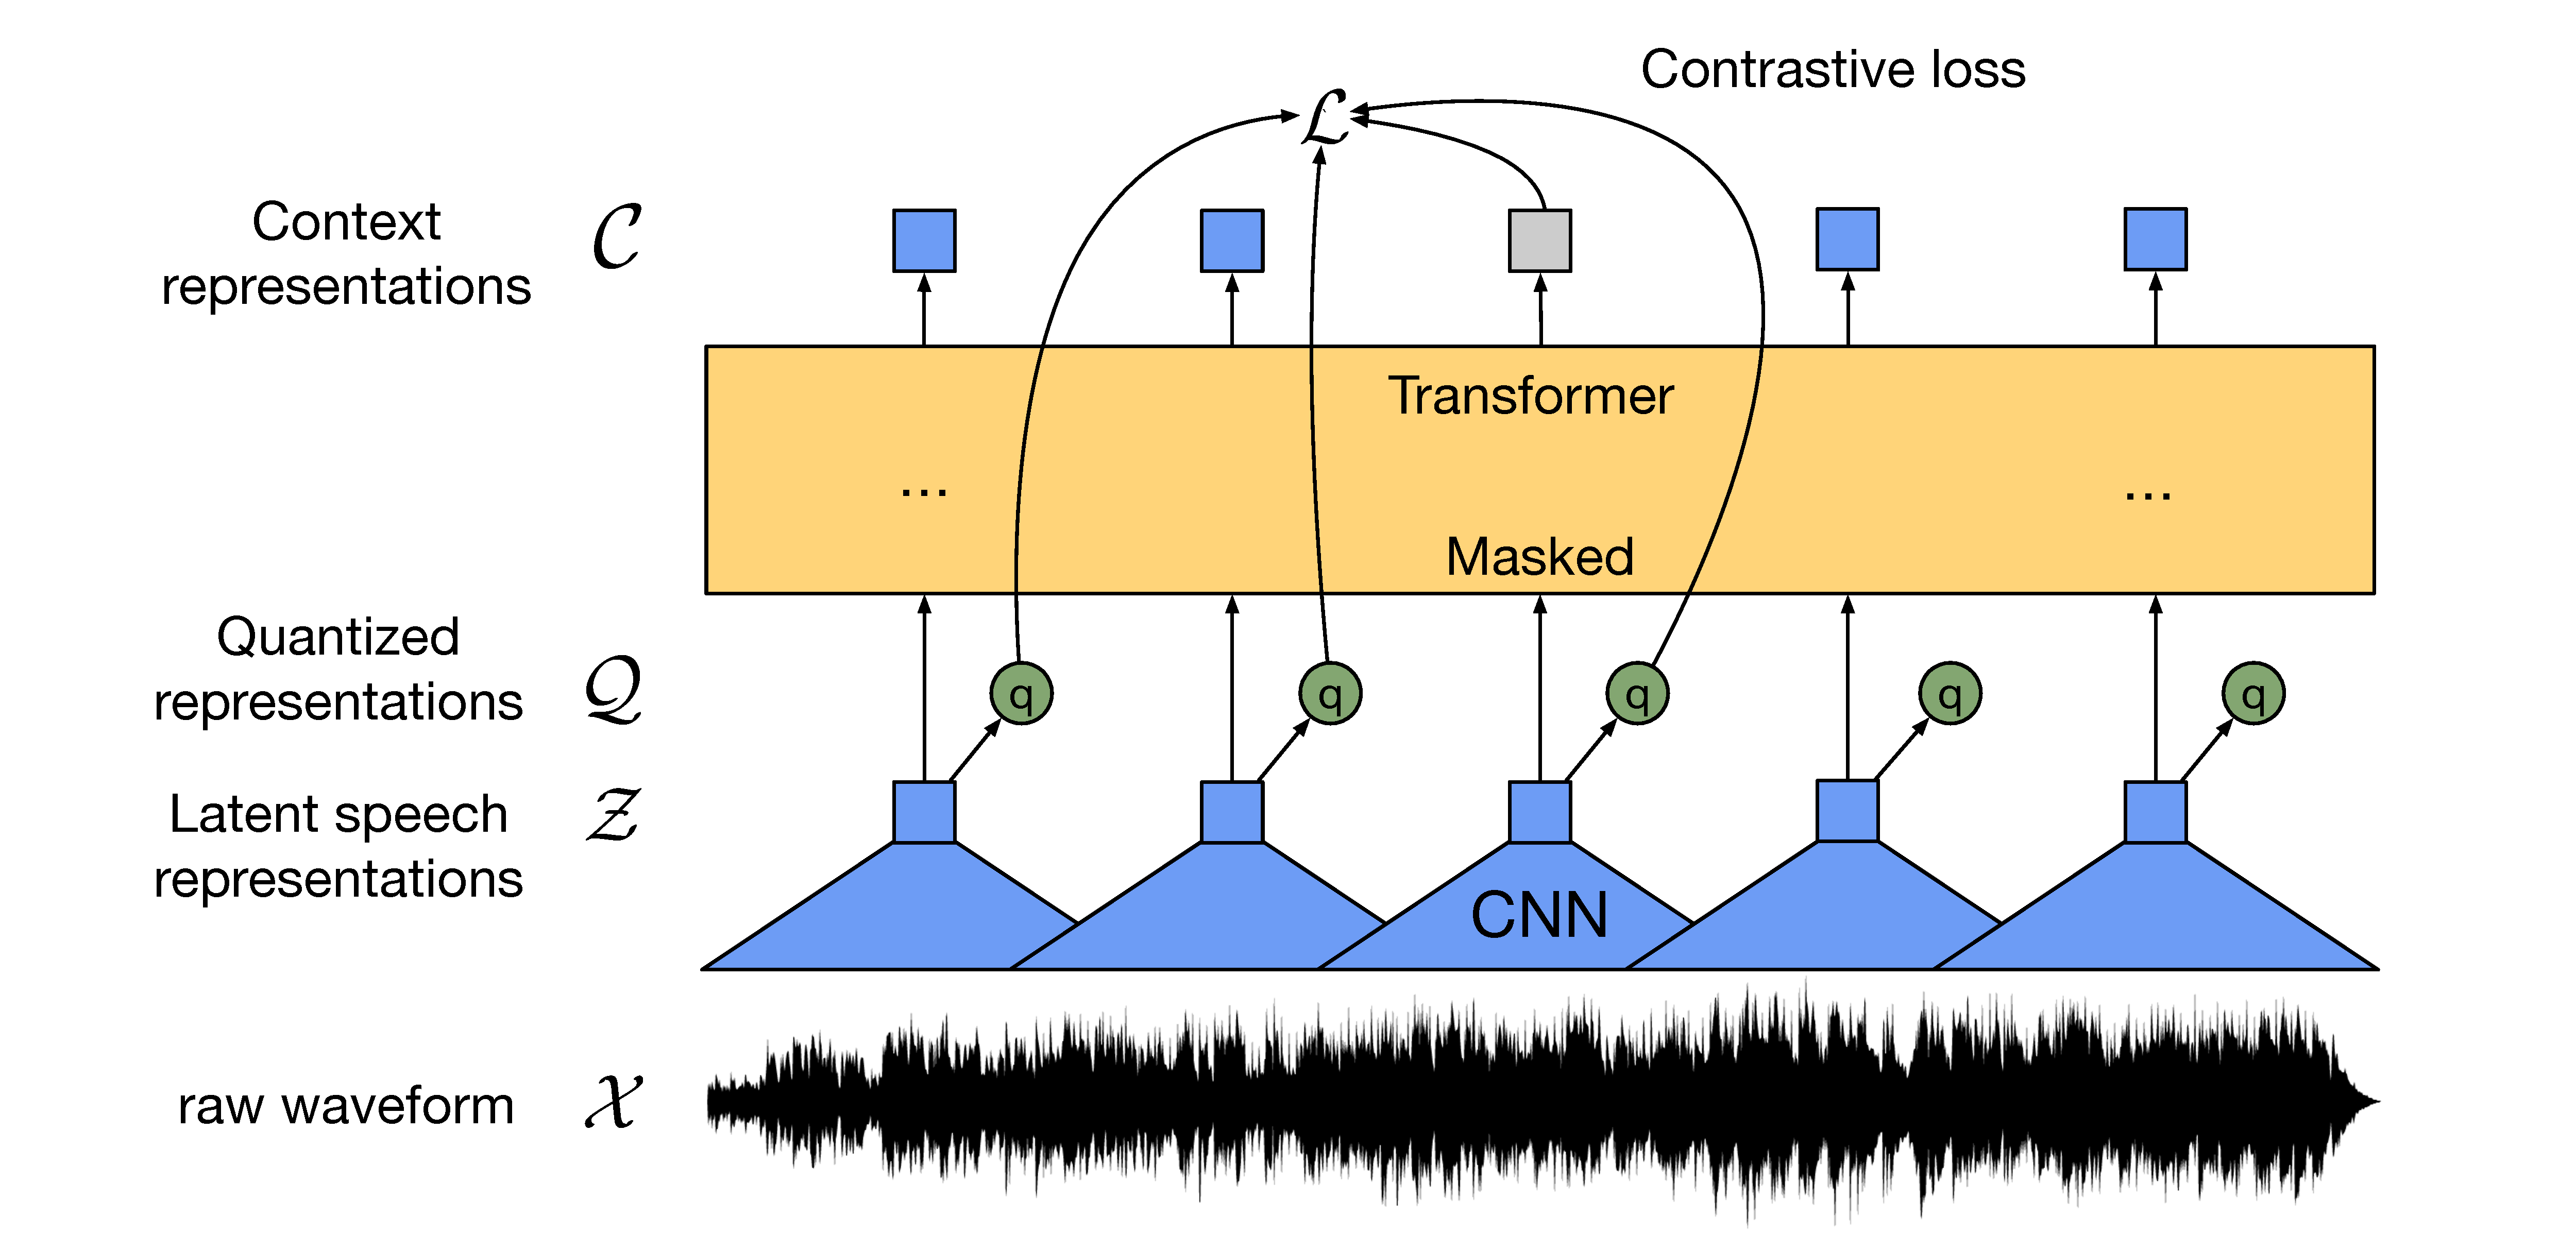
\includegraphics[width=\textwidth]{illustration.pdf}
    \caption{A visualization of the network architecture of wav2vec 2.0 \cite{baevski2020wav2vec}.}
    \label{wav2vec2_architecture}
\end{figure}



\subsection{Feature encoder}
The feature encoder maps the raw audio data (speech recordings) to latent speech representations: $f: \mathcal{X} \rightarrow \mathcal{Z}$.
Thus, the feature encoder $f$ maps a sequence of audio samples $\mathbf{x}^{(1)}, \dots \mathbf{x}^{(N)}$ into a sequence of latent feature vectors $\mathbf{z}^{(1)}, \dots, \mathbf{z}^{(t)}$.
% Explain the purpose of feature encoder

The audio data is scaled to have zero mean and unit variance before going into the feature encoder. 
The feature encoder consists of seven convolutional blocks, where each convolutional block contains a temporal\footnote{One-dimensional convolutional layer designed for sequential data.} convolutional layer, 
a layer normalization layer, and the GELU activation function.

Each temporal convolutional layer contains 512 channels. 
The strides of the seven temporal convolutional layers are $(5,2,2,2,2,2,2)$ and the kernel widths are $(10,3,3,3,3,2,2)$.
The strides used results in each $\mathbf{z}^{(t)}$ representing $25$ms of audio (or $400$ input samples),
strided by about $20$ms.

Layer normalization scales the logits after each convolutional layer to have zero mean and unit variance, which has shown to increase the chances of earlier convergence.
GELU has become a popular activation function for NLP related tasks



\subsection{Quantization module}
The quantization module maps the latent speech features into discrete speech units: $h: \mathcal{Z} \rightarrow \mathcal{Q}$.
Speech is sound, and sound is represented as a continuous function. We would like to use Transformers and so continuous representations will not work. 
Unlike written language, which can be discretized into tokens such as characters or sub-words, speech does not have natural sub-units \cite{bgn2021illustrated}. 
The quantization module is a method in which discrete speech units are automatically learned using product quantization.

To perform product quantization, the quantization module uses $G$ \emph{codebooks}, where each codebook contains $V$ \emph{codebook entries} $\mathbf{e}_{1}, \dots, \mathbf{e}_{V}$.

The following steps describe the process of automatically assigning a discrete speech unit to each latent speech feature $\mathbf{z}^{(t)}$:
\begin{enumerate}
    \item Transform $\mathbf{z}^{(t)}$ into $\mathbf{l}^{(t)} \in \mathbb{R}^{G \times V}$ using a linear transformation.
    \item Choose one codebook entry $\mathbf{e}_g$ for each codebook $g = 1, \dots, G$, based on the values of $\mathbf{l}^{(t)}$.
    \item Concatenate the codebook entries $\mathbf{e}_1, \dots, \mathbf{e}_G$.
    \item Transform the resulting vector into $\mathbf{q}^{(t)} \in \mathbb{R}^{f}$ using another linear transformation.
\end{enumerate}
The two linear transformations are feed-forward neural networks $\text{FF}_1: \mathbb{R}^{f} \rightarrow \mathbb{R}^{G \times V}$ and $\text{FF}_2: \mathbb{R}^{d} \rightarrow \mathbb{R}^{f}$.
In the second step above, the codebook entry $\mathbf{e}_g$ is chosen as the one with the argmax of the logits $\mathbf{l}$. Choosing the codebook entries in this way is non-differentiable.
Fortunately, we can use the Gumbel softmax to choose codebook entries in a fully differentiable way. 
$\mathbf{e}_g$ is chosen as the entry that maximizes
\begin{equation}
    p_{g, v} = \dfrac{\exp{\left(\mathbf{l}^{(t)}_{g, v} + n_v\right)}/\tau}{\sum\limits_{k=1}^{V} \exp{\left(\mathbf{l}^{(t)}_{g, k} + n_k\right)}/\tau},
\end{equation}
where $\tau$ is a non-negative temperature, $n = -\log{(-\log{(u)})}$, and $u$ are uniform samples from $\mathcal{U}(0, 1)$.
During the forward pass, codeword $i$ is chosen by $i = \text{argmax}_j p_{g,j}$ and in the backward pass, the true gradient of the Gumbel softmax outputs is used.



\subsection{Context network}
% Explain what it is and its purpose
The context network creates contextualized representations from the feature encoder outputs.
The main component of the context network is a Transformer encoder \cite{transformer}.
Due to the popularity of Transformers we have ommited a detailed explanation of the Transformer architecture. 
Interested readers should refer to \cite{transformer} as well as guides such as \cite{alammar2018illustrated}.

% Explain architecture further
The following steps describe how the latent feature vectors are processed before being fed into the Transformer encoder.
\begin{enumerate}
    \item The latent feature vectors are fed into a \emph{feature projection layer} to match the model dimension of the context network.
    \item Positional embedding vectors are added to the inputs using \emph{relative positional encoding} \cite{shaw2018relative} instead of absolute positional encoding.
    The relative positional encoding is implemented using grouped convolution \cite{AlexNet}.
    \item Inputs are fed into the GELU activation function, followed by layer normalization.
\end{enumerate}

% Absolute position embeddings encode the absolute position of a word in the input phrase, the first word has position 1, 
% the 50th word has position 50. Relative position embeddings encode the relative position two words have to each other, 
% so the relative position between words 7 and 10 in a phrase would be 3.

% Explain LARGE Transformer encoder structure
The details for the Transformer encoder of the \textsc{LARGE} version of wav2vec 2.0 is as follows:
\begin{itemize}
    \item Numer of Transformer blocks: $B = 24$.
    \item Model dimension: $H_m = 1024$.
    \item Inner dimension: $H_{ff} = 4096$.
    \item Numer of attention heads: $A = 16$.
\end{itemize}



\subsection{Pretraining with wav2vec 2.0}

\paragraph*{Masking.}
In Wav2Vec 2.0, the masking process plays a crucial role in pretraining. 
It involves two hyperparameters: $p = 0.065$ and $M = 10$. 
The masking is performed as follows:
\begin{enumerate}
    \item All time steps from the latent speech representation space $Z$ are considered.
    \item A proportion $p$ of vectors from the previous step is sampled without replacement. These sampled vectors determine the starting indices.
    \item For each starting index $i$, consecutive $M$ time steps are masked. There may be overlap between these masked spans.
\end{enumerate}

\paragraph*{Training objective.} There are two objectives (loss functions) that wav2vec 2.0 optimizes simultaneously.
The first loss function is the contrastive loss $\mathcal{L}_m$ which encourages the model to
identify the true quantized representation for a masked time step within a set of distractors. 
The second loss function is the diversity loss $\mathcal{L}_d$ which encourages the model 
to equally use the codebook entries from the quantization module.
The full training objective is given by
\begin{equation}
\mathcal{L} = \mathcal{L}_m + \alpha \mathcal{L}_d,
\end{equation}
where $\alpha$ is a tuned hyperparameter.

\paragraph*{Contrastive loss.}
The contrastive loss is responsible for training the model to predict the correct quantized 
representation $\mathbf{q}_t$ from a set of candidate representations $\mathbf{\tilde{q}} \in \mathcal{Q}_t$. 
The set $\mathcal{Q}_t$ includes the target $\mathbf{q}_t$ and $K$ distractors sampled uniformly from other masked time steps. 
The contrastive loss is given by
\begin{equation}
\mathcal{L}_m = -\log \dfrac{\exp(\text{sim}(\mathbf{c_t}, \mathbf{q_t}) \/ \kappa)}{\sum_{\mathbf{\tilde{q}} \sim \mathcal{Q}_t} \exp(\text{sim}(\mathbf{c_t}, \mathbf{\tilde{q}}) \/ \kappa)},
\end{equation}
where $\kappa$ represents a constant temperature, and $\text{sim}(a, b)$ denotes the cosine similarity between 
context representation $c_t$ and quantized representations $q$. 
This loss encourages the model to assign high similarity to the true 
positive target and penalize high similarity with negative distractors.

\paragraph*{Diversity loss.}
The diversity loss is a regularization technique aimed at promoting the equal use of codebook entries. 
It is based on entropy and is calculated as:
\begin{equation}
    \mathcal{L}_d = \dfrac{1}{GV}\sum_{g=1}^{G} -H(\bar{p}_{g}) = -\dfrac{1}{GV}\sum_{g=1}^{G} \sum_{v=1}^{V} \bar{p}_{g,v} \log \bar{p}_{g,v}
\end{equation}
This loss maximizes the entropy of the softmax distribution $\bar{p}_{g,v}$ over codebook entries, encouraging the model to utilize all code words equally.



\subsection{Fine-tuning with wav2vec 2.0}
There are three steps required to fine-tune a pretrained wav2vec 2.0 model for automatic speech recognition:
\begin{enumerate}
    \item Prepare a labeled dataset - a corpus of speech recordings with corresponding transcriptions.
    \item Replace the head of the model with a linear layer that has an equal number of output neurons as the number of
    characters in the set of characters of the transcription data.
    \item Optimize the model using the Connectionist Temporal Classification (CTC) loss function.
\end{enumerate}



% ***************************************************
% SECTION 3
% ***************************************************
\section{Connectionist Temporal Classification}
Connectionist Temporal Classification (CTC) \cite{graves2006connectionist} is a loss function (and an algorithm)
developed to map a sequence of speech features to a sequence of characters.
Our explanation of CTC is heavily based on the automatic speech recognition chapter in \cite{jurafskyspeech}.
We recommend readers to use Figure~\ref{ctc} as a visual aid for our explanation.

\begin{figure}
    \centering
    \captionsetup{justification=centering}
    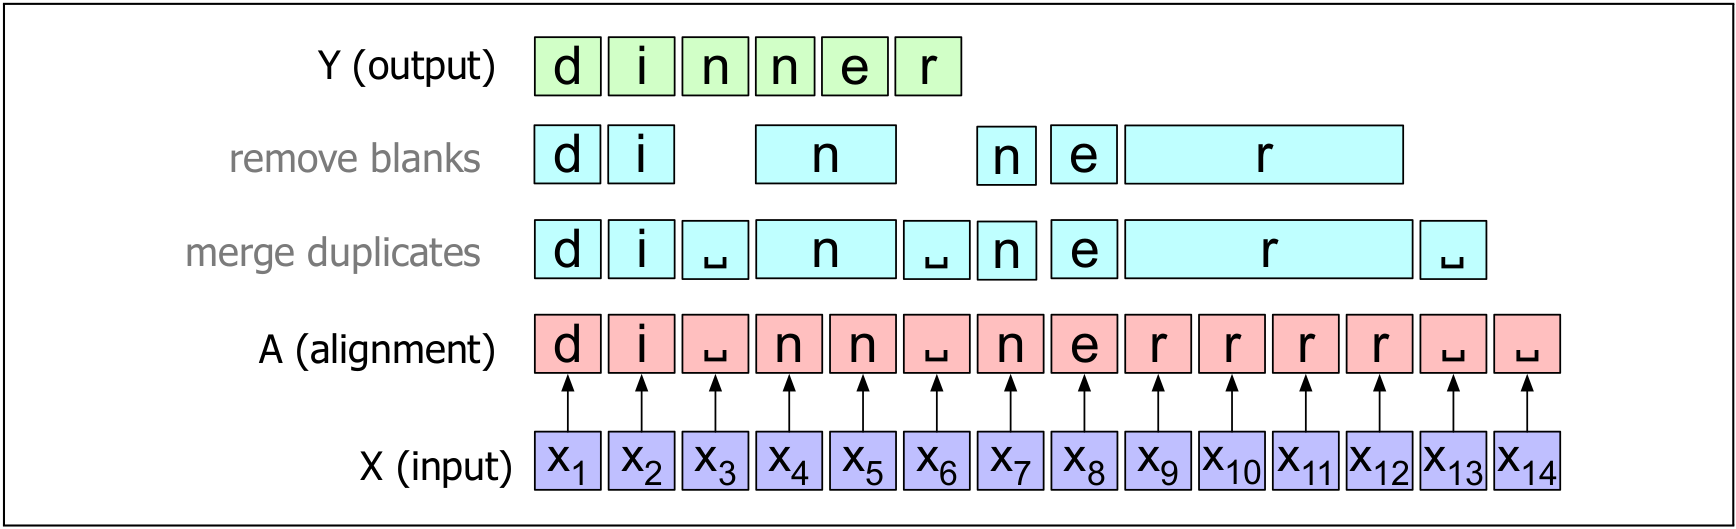
\includegraphics[width=\textwidth]{ctc.png}
    \caption{A diagram that describes the alignment procedure of CTC \cite{jurafskyspeech}.}
    \label{ctc}
\end{figure}

Given a sequence of speech features, CTC maps each speech feature to a single character to form a sequence of characters called an \emph{alignment}. 
Then, a \emph{collapsing function} is used to remove consecutive duplicate characters in the alignment to form an output string (the predicted transcription).
The authors of CTC propose the use of a special characters called a \emph{blank}, which is represented by \textvisiblespace.
The blank character accounts for words that contain consecutive duplicate characters (such as ``dinner'' which contains two consecutive ``n'' characters).
With the addition of the blank character, the collapsing function is responsible for removing consecutive duplicate characters and removing all instances of blank characters.
Following the notation of \cite{jurafskyspeech}, we define the collapsing function as a mapping $B: a \rightarrow y$ for an alignment $a$ and output string $y$.
Notice that $B$ is many-to-one, since many different alignments can map to the same ouptut string (see Figure~\ref{dinner}).

\begin{figure}
    \centering
    \captionsetup{justification=centering}
    
\includegraphics[width=\textwidth]{dinner.png}
    \caption{Three different alignments that produce the same output string when using the CTC collapsing function \cite{jurafskyspeech}.}
    \label{dinner}
\end{figure}

In \cite{jurafskyspeech}, the set of all alignments that map to the same output string is denoted as $B^{-1}(Y)$, 
where $B^-1$ is the inverse of the collapsing function and $Y$ is an output string.
This notation is useful for our explanation of CTC inference and training.

\subsection{CTC Inference}
Here we discuss how CTC computes $P_{\text{CTC}(Y|X)}$ which denotes the probability of 
the output string $Y$ for an input sequence of speech features $X = \{x^{(1)}, \dots, x^{(T)}\}$.
Notice that $P_{\text{CTC}(Y|X)}$ can be rewritten as $P_{\text{CTC}(Y|X)} = \sum\limits_{A \in B^{-1}(Y)} P(A|X)$, 
which is the sum the probabilities of all possible alignments that produce the output string $Y$.

CTC makes a strong conditional independence to obtain an expression $P(A|X)$. 
It assumes that the probability of each alignment character $a^{(t)} \in \{a^{(1)}, \dots, a^{(T)}\}$
is computed independently of all the other alignment characters: $P(A|X) = \prod\limits_{t=1}^{T} p(a^{(t)} | X)$.
Thus we can find the best possible alignment for a given $X$ by choosing the most probable character at each time step
using the argmax operator: $a^{(t)} = \text{argmax}_{c \in \mathcal{C}} p_{t}(c|X)$, where $\mathcal{C}$ represents the
vocabulary.

% TODO change
There is a flaw with the greedy approach described above. The problem is that we chose the most likely alignment A, but the
most likely alignment may not correspond to the most likely final collapsed output
string Y. That's because there are many possible alignments that lead to the same
output string, and hence the most likely output string might not correspond to the
most probable alignment.

% TODO change
For this reason, the most probable output sequence $\hat{Y}$ is the one that has, not
the single best CTC alignment, but the highest sum over the probability of all its
possible alignments:

\begin{equation}
    P_{\text{CTC}}(Y|X) =  \sum\limits_{A \in B^{-1}(Y)} P(A|X) = \sum\limits_{A \in B^{-1}(Y)} \prod\limits_{t=1}^{T} p(a^{(t)} | X)
\end{equation}
    
\begin{equation}
\hat{Y} = \text{argmax}_Y P_{\text{CTC}}(Y|X)
\end{equation}

% TODO change
Alas, summing over all alignments is very expensive, because there are many possible alignments.
We use dynamic programming to approximate this sum by using a modified version of Viterbi beam search that cleverly
keeps in the beam the high-probability alignments that map to the same output string,
and sums those as an approximation of the equation above.

\paragraph*{Improving CTC with a LM.} Because of the strong conditional independence assumption mentioned earlier,
CTC does not implicitly learn a language model over the data (unlike the attentionbased encoder-decoder architectures). It is therefore essential when using CTC to
interpolate a language model using interpolation weights that are tuned on a validation set:

\begin{equation}
    \textit{score}_{\text{CTC}}(Y|X) = \log\left(P_{\text{CTC}}(Y|X)\right) + \lambda_1 \log\left(P_{\text{LM}}(Y)\right) + \lambda_2 L(Y)
\end{equation}
    

\subsection{CTC Training}
TODO
% Write about $n$-gram models, Kneser-Nay, and stuff



% ***************************************************
% SECTION 4
% ***************************************************
\section{Pretrained wav2vec 2.0 models}
TODO: Explain why I can't perform pretraining

\subsection{XLS-R}
TODO: Provide high-level overview.
